\documentclass{article}
\usepackage{graphicx}
\usepackage{booktabs}
\usepackage{amsmath}
\begin{document}
% formula_001
\[Y ^ { \prime } [ h , w , c ] = \sum _ { i = 0 } ^ { D _ { h } - 1 } \sum _ { j = 0 } ^ { D _ { w } - 1 } X [ h + i , w + j , c ] \cdot F _ { \text {depthwise} } [ i , j , c ] , \\ \intertext { f o r e a c h s p o r i l $ o r $ t i n t i o n } ( h _ { \ } w ) _ { \ } a n d \text { channel } _ { \ } T h i s \text { opera}\]

% formula_002
\[Y [ h , w , p ] = \sum _ { c = 0 } ^ { C - 1 } Y ^ { \prime } [ h , w , c ] \cdot F _ { \text {pointwise} } [ 1 , 1 , c , p ] , \quad ( 2 ) \ \text {ability}\]

% formula_003
\[Z _ { i } = S _ { i } ^ { \prime } + X _ { i } ^ { \prime } .\]

% formula_004
\[\tilde { Z } _ { i } = B N ( \sigma ( \text {Conv} ( Z _ { i } ) ) ) \, ,\]

% formula_005
\[\intertext { s i n t w i s e } \intertext { s i n t w i s e } \intertext { s i n t w i s e } \intertext { s i n t w i s e } \intertext { s i n t w i s e } \intertext { s i n t w i s e } \intertext { s i n t w i s e } \intertext { s i n t w i s e } \intertext { s i n t w i s e } \intertext { s i n t w i s e } \intertext { s i n t w i s e } \intertext { s i n t w i s e } \intertext { s i n t w i s e } \intertext { s i n t w i s e } \intertext { s i n t w i s e } \intertext { s i n t w i s e } \intertext { s i n t w i s e } \intertext { s i n t w i s e } \intertext { s i n t w i s e } \intertext { s i n t w i s e } \intertext { s i n t w i s e } \intertext { s i n t w i s e } \intertext { s i n t w i s e } \intertext { s i n t w i s e } \intertext { s i n t w i s e } \intertext { s i n t w i s e } \intertext { s i n t w i s e } \intertext { s i n t w i s e } \intertext { s i n t w i s e } \intertext { s i n t w i s e } \intertext { s i n t w i s e } \intertext { s i n t w i s e } \intertext { s i n t w i s e } \intertext { s i n t w i s e } \intertext { s i n t w i s e } \intertext { s i n t w i s e } \intertext { s i n t w i s e } \intertext { s i n t w i s e } \intertext { s i n t w i s e } \intertext { s i n t w i s e } \intertext { s i n t w i s e } \intertext { s i n t w i s e } \intertext { s i n t w i s e } \intertext { s i n t w i s e } \intertext { s i n t w i s e } \intertext { s i n t w i s e } \intertext { s i n t w i s e } \intertext { s i n t w i s e } \intertext { s i n t w i s e } \intertext { s i n t w i s e } \intertext { s i n t w i s e } \intertext { s i n t w i s e } \intertext { s i n t w i s e } \intertext { s i n t w i s e } \intertext { s i n t w i s e } \intertext { s i n t w i s e } \intertext { s i n t w i s e } \intertext { s i n t w i s e } \intertext { s i n t w i s e } \intertext { s i n t w i s e } \intertext { s i n t w i s e } \intertext { s i n t w i s e } \intertext { s i n t w i s e } \intertext { s i n t w i s e } \intertext { s i n t w i s e } \intertext { s i n t w i s e } \intertext { s i n t w i s e } \intertext { s i n t w i s e } \intertext { s i n t w i s e } \intertext { s i n t w i s e } \intertext { s i n t w i s e } \intertext { s i n t w i s e } \intertext { s i n t w i s e } \intertext { s i n t w i s e } \intertext { s i n t w i s e } \intertext { s i n t w i s e } \intertext { s i n t w i s e } \intertext { s i n t w i s e } \intertext { s i n t w i s e } \intertext { s i n t w i s e } \intertext { s i n t w i s e } \intertext { s i n t w i s e } \intertext { s i n t w i s e } \intertext { s i n t w i s e } \intertext { s i n t w i s e } \intertext { s i n t w i s e } \intertext { s i n t w i s e } \intertext { s i n t w i s e } \intertext { s i n t w i s e } \intertext { s i n t w i s e } \intertext { s i n t w i s e } \intertext { s i n t w i s e } \intertext { s i n t w i s e } \intertext { s i n t w i s e } \intertext { s i n t w i s e } \intertext { s i n t w i s e } \intertext { s i n t w i s e } \intertext { s i n t w i s e } \intertext { s i n t w i s e } \intertext { s i n t w i s e } \intertext { s i n t w i s e } \intertext { s i n t w i s e } \intertext { s i n t w i s e } \intertext { s i n t w i s e } \intertext { s i n t w i s e } \intertext { s i n t w i s e } \intertext { s i n t w i s e } \intertext { s i n t w i s e } \intertext { s i n t w i s e } \intertext { s i n t w i s e } \intertext { s i n t w i s e } \intertext { s i n t w i s e } \intertext { s i n t w i s e } \intertext { s i n t w i s e } \intertext { s i n t w i s e } \intertext { s i n t w i s e } \intertext { s i n t w i s e } \intertext { s i n t w i s e } \intertext { s i n t w i s e } \intertext { s i n t w i s e } \intertext { s i n t w i s e } \intertext { s i n t w i s e } \intertext { s i n t w i s e } \intertext { s i n t w i s e } \intertext { s i n t w i s e } \intertext { s i n t w i s e } \intertext { s i n t w i s e } \intertext { s i n t w i s e } \intertext { s i n t w i s e } \intertext { s i n t w i s e } \intertext { s i n t w i s e } \intertext { s i n t w i s e } \intertext { s i n t w i s e } \intertext { s i n t w i s e } \intertext { s i n t w i s e } \intertext { s i n t w i s e } \intertext { s i n t w i s e } \intertext { s i n t w i s e } \intertext { s i n t w i s e } \intertext { s i n t w i s e } \intertext { s i n t w i s e } \intertext { s i n t w i s e } \intertext { s i n t w i s e } \intertext { s i n t w i s e } \intertext { s i n t w i s e } \intertext { s i n t w i s e } \intertext { s i n t w i s e } \intertext { s i n t w i s e } \intertext { s i n t w i s e } \intertext { s i n t w i s e } \intertext { s i n t w i s e } \intertext { s i n t w i s e } \intertext { s i n t w i s e } \intertext { s i n t w i s e } \intertext { s i n t w i s e } \intertext { s i n t w i s e } \intertext { s i n t\]

% formula_006
\[\hat { p } _ { x - y } ^ { M } = f _ { x - y } ( A _ { x - y } ^ { M } ) \, ,\]

% formula_007
\[\hat { p } _ { y - z } ^ { M } = f _ { y - z } \left ( S _ { y - z } ^ { M } \right ) ,\]

% formula_008
\[\hat { p } _ { x - z } ^ { M } = f _ { x - z } \left ( C _ { x - z } ^ { M } \right ) .\]

% formula_009
\[\hat { P } ^ { M } = \frac { \hat { p } _ { x - y } ^ { M } + \hat { p } _ { y - z } ^ { M } + \hat { p } _ { x - z } ^ { M } } { 3 } .\]

% formula_010
\[P ^ { M } = T ( \hat { P } ^ { M } ) = \begin{cases} 1 , & \hat { P } ^ { M } \geq 0 . 5 , \\ 0 , & \text {otherwise} . \end{cases}\]

% formula_011
\[\alpha i a l \colon [ 0 , 200 , 500 , 1 0 0 , 2 0 0 , 3 0 0 , \infty ) , \\ s a g i t t a l \colon [ 0 , 500 , 1 0 0 , 2 0 0 , 3 0 0 , 5 0 0 , \infty ) , \\ c o r n a l \colon [ 0 , 200 , 500 , 1 0 0 , 2 0 0 , 3 0 0 , \infty ) .\]

% formula_012
\[\text {Precision} = \frac { T P } { T P + F P } , & & ( 4 a ) \\\]

% formula_013
\[R e c a l l = \frac { T P } { T P + F N } ,\]

% formula_014
\[\ D S C = \frac { 2 \, T P } { 2 \, T P + F P + F N } .\]

% formula_015
\[\L _ { F L } = - \frac { 1 } { | \Omega | } \sum _ { v \in \Omega } \left [ \alpha _ { f } \, g _ { v } \left ( 1 - p _ { v } \right ) ^ { \gamma _ { f } } \log p _ { v } \\ \intertext { s t r i b u - } \int e x t { f } = 0 \quad + ( 1 - \alpha _ { f } ) \left ( 1 - g _ { v } \right ) p _ { v } ^ { \gamma _ { f } } \log ( 1 - p _ { v } ) \right ] . \\ \intertext { a k a g e . } \int e x t { 5 } \quad ( 5 )\]

% formula_016
\[\text {TI} ( p , g ) & = \frac { \sum _ { v } p _ { v } g _ { v } } { \sum _ { v } p _ { v } g _ { v } + \alpha _ { t } \sum _ { v } ( 1 - g _ { v } ) p _ { v } + \beta _ { t } \sum _ { v } g _ { v } ( 1 - p _ { v } ) } , \\ \text {with } & \sum _ { ( 6 ) } p _ { 1 } \varrho _ { v } \text {, with } \text { } F D _ { v } \text {, } \text { } F N _ { v } \text {, } \text { } \text { } \text { } T h s c r { C }\]

% formula_017
\[\mathcal { L } _ { T L } = 1 - T I ( p , g ) .\]

% formula_018
\[\mathcal { L } _ { F T } = \lambda \, \mathcal { L } _ { T L } + ( 1 - \lambda ) \, \mathcal { L } _ { F L } ,\]

\begin{table}[htbp]
\centering
\label{tab:table\_001}
\begin{tabular}{llllll}
\hline
One Lesion &  &  & Multiple Lesions &  &  \\
\hline
Left & Right & Other & Unilateral & Bilateral & Other \\
Data 173 (26.4\%) & 187 (28.5\%) & 46 (7.0\%) & 47 (7.2\%) & 121 (18.5\%) & 81 (12.4\%) \\
\hline
\end{tabular}
\end{table}

\begin{table}[htbp]
\centering
\caption{TABLE II LESION COUNT AND LOCATION IN CORTICAL AND SUBCORTICAL REGIONS OF THE ATLAS V2.0 DATASET}
\label{tab:table\_002}
\begin{tabular}{lllllll}
\hline
One Lesion &  &  & Multiple Lesions &  & Others & Total \\
\hline
 & Left & Right & Left & Right &  &  \\
Data & 132 (12.0\%) & 149 (13.5\%) & 333 (30.2\%) & 324 (29.4\%) & 163 (14.8\%) & 1101 \\
\hline
\end{tabular}
\end{table}

\begin{table}[htbp]
\centering
\caption{TABLE III PERFORMANCE OF DIFFERENT LOSS FUNCTIONS ON THE FIRST AXIAL FOLD}
\label{tab:table\_003}
\begin{tabular}{lllll}
\hline
Loss Function & Dice & Precision & Recall & F1 \\
\hline
Dice Loss & 0.7859 & 0.8430 & 0.7406 & 0.7889 \\
Focal Loss & 0.7326 & 0.7302 & 0.7427 & 0.7364 \\
Tversky Loss & 0.7764 & 0.7559 & 0.8037 & 0.7791 \\
FocalTversky (Proposed) & 0.7904 & 0.7963 & 0.7894 & 0.7928 \\
\hline
\end{tabular}
\end{table}

\begin{table}[htbp]
\centering
\caption{TABLE IV FIVE-FOLD PERFORMANCE OF THE PROPOSED MODEL ON AXIAL, SAGITTAL, AND CORONAL PLANES}
\label{tab:table\_004}
\begin{tabular}{lllll}
\hline
Plane & Fold & Dice & Precision & Recall \\
\hline
Axial & 1 2 3 4 5 Avg & 0.6878 ± 0.3762 0.7047 ± 0.3792 0.7282 ± 0.3558 0.7209 ± 0.3684 0.7104 ± 0.3776 0.7104 ± 0.0127 & 0.7713 ± 0.3324 0.8391 ± 0.2832 0.8269 ± 0.2808 0.8515 ± 0.2678 0.8638 ± 0.2559 0.8305 ± 0.0292 & 0.8055 ± 0.3291 0.7674 ± 0.3606 0.7958 ± 0.3355 0.7753 ± 0.3533 0.7567 ± 0.3675 0.7801 ± 0.0164 \\
Sagittal & 1 2 3 4 5 Avg & 0.6260 ± 0.3996 0.6058 ± 0.4159 0.6527 ± 0.3947 0.6178 ± 0.3992 0.6063 ± 0.3989 0.6217 ± 0.0157 & 0.7838 ± 0.3313 0.8236 ± 0.3064 0.8305 ± 0.2841 0.7492 ± 0.3447 0.7346 ± 0.3537 0.7843 ± 0.0350 & 0.6931 ± 0.3889 0.6685 ± 0.4100 0.7062 ± 0.3879 0.7302 ± 0.3781 0.7297 ± 0.3738 0.7055 ± 0.0212 \\
Coronal & 1 2 3 4 5 Avg & 0.6579 ± 0.3990 0.6918 ± 0.3802 0.6932 ± 0.3843 0.6994 ± 0.3810 0.6953 ± 0.3861 0.6875 ± 0.0137 & 0.7844 ± 0.3301 0.8161 ± 0.3033 0.8512 ± 0.2704 0.8376 ± 0.2874 0.8701 ± 0.2519 0.8319 ± 0.0269 & 0.7605 ± 0.3735 0.7665 ± 0.3569 0.7451 ± 0.3769 0.7620 ± 0.3627 0.7402 ± 0.3801 0.7549 ± 0.0093 \\
\hline
\end{tabular}
\end{table}

\begin{table}[htbp]
\centering
\caption{TABLE VI AVERAGE TRAINING TIME, PER-SLICE PREDICTION TIME, AND}
\label{tab:table\_005}
\begin{tabular}{llllll}
\hline
Plane & Model & Dice & Precision & Recall & F1 \\
\hline
Axial & X-Net CLCI RAX & 0.6606 0.5904 0.7104 & 0.9506 0.9760 0.8305 & 0.6590 0.5864 0.7801 & 0.7796 0.7310 0.8045 \\
Sagittal & X-Net CLCI RAX & 0.6103 0.5830 0.6217 & 0.9216 0.9000 0.7843 & 0.6165 0.6002 0.7055 & 0.7375 0.7200 0.7429 \\
Coronal & X-Net CLCI RAX & 0.6439 0.5721 0.6875 & 0.9585 0.6928 0.8319 & 0.6382 0.5774 0.7549 & 0.7666 0.6298 0.7913 \\
\hline
\end{tabular}
\end{table}

\begin{table}[htbp]
\centering
\label{tab:table\_006}
\begin{tabular}{lllll}
\hline
Plane & Model & Training Time (h) & Prediction Time (s) & Parameters \\
\hline
Axial & X-Net CLCI & 8.98 3.91 1.02 & 0.0520 0.0590 0.0418 & 15,072,332 36,813,025 4,829,665 \\
 & RAX &  &  &  \\
Sagittal & X-Net & 11.76 & 0.0540 & 15,072,332 \\
 & CLCI & 8.94 & 0.0620 & 36,813,025 \\
 & RAX & 1.75 & 0.0417 & 4,829,665 \\
Coronal & X-Net & 9.50 & 0.0520 & 15,072,332 \\
 & CLCI & 2.96 & 0.0980 & 36,813,025 \\
 & RAX & 1.31 & 0.0407 & 4,829,665 \\
\hline
\end{tabular}
\end{table}

\begin{table}[htbp]
\centering
\caption{TABLE VII PER-PLANE PERFORMANCE BEFORE AND AFTER AGGREGATION ON 112 CASES}
\label{tab:table\_007}
\begin{tabular}{lllll}
\hline
Plane & Aggregation & Dice & Precision & Recall \\
\hline
Axial & No & 0.8016 0.8451 & 0.8612 0.9019 & 0.8748 0.8807 \\
 & Yes &  &  &  \\
Sagittal & No & 0.8231 & 0.8830 & 0.8951 \\
 & Yes & 0.8753 & 0.9331 & 0.9022 \\
Coronal & No & 0.8184 & 0.8984 & 0.8712 \\
 & Yes & 0.8633 & 0.9156 & 0.8987 \\
\hline
\end{tabular}
\end{table}

\begin{table}[htbp]
\centering
\caption{TABLE VIII SUBJECT-LEVEL RESULTS ON 112 3D MRI CASES (AGGREGATED PREDICTIONS)}
\label{tab:table\_008}
\begin{tabular}{llll}
\hline
Dice & Precision & Recall & Volume Difference \\
\hline
0.6126 ± 0.2577 & 0.6833 ± 0.2281 & 0.6385 ± 0.2963 & 6486 ± 9686 \\
\hline
\end{tabular}
\end{table}

\begin{table}[htbp]
\centering
\caption{TABLE IX EFFECT OF RESIDUAL CONNECTIONS ON SEGMENTATION PERFORMANCE (SAGITTAL, FOLD 3)}
\label{tab:table\_009}
\begin{tabular}{lllll}
\hline
 & Dice & Precision & Recall & F1 \\
\hline
With residual & 0.6260 & 0.7838 & 0.6931 & 0.7356 \\
Without residual & 0.5951 & 0.8070 & 0.6403 & 0.7147 \\
\hline
\end{tabular}
\end{table}

% Figure assets are relative to the package root.
\begin{figure}[htbp]
\centering

\includegraphics[width=0.9\linewidth]{../figures/figure_001.png}
\caption{}
\end{figure}
\begin{figure}[htbp]
\centering
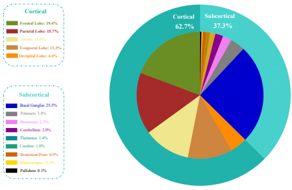
\includegraphics[width=0.9\linewidth]{../figures/figure_002.png}
\caption{Fig. 1. Distribution of ischemic stroke lesions across cortical and subcortical regions in the ATLAS v2.0 dataset.}
\end{figure}
\begin{figure}[htbp]
\centering
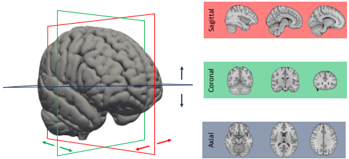
\includegraphics[width=0.9\linewidth]{../figures/figure_003.png}
\caption{Fig. 2. Decomposition of a 3D MRI scan into axial, sagittal, and coronal planes. Blue, red, and green rectangles indicate the superior-inferior (axial), anterior-posterior (sagittal), and left-right (coronal) axes, respectively.}
\end{figure}
\begin{figure}[htbp]
\centering
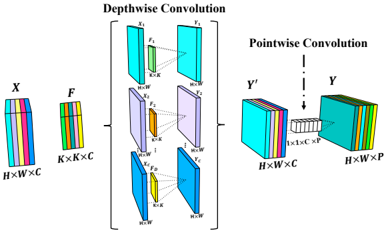
\includegraphics[width=0.9\linewidth]{../figures/figure_004.png}
\caption{Fig. 3. Illustration of the separable convolution architecture, showing the decomposition of standard convolution into depthwise and pointwise operations.}
\end{figure}
\begin{figure}[htbp]
\centering
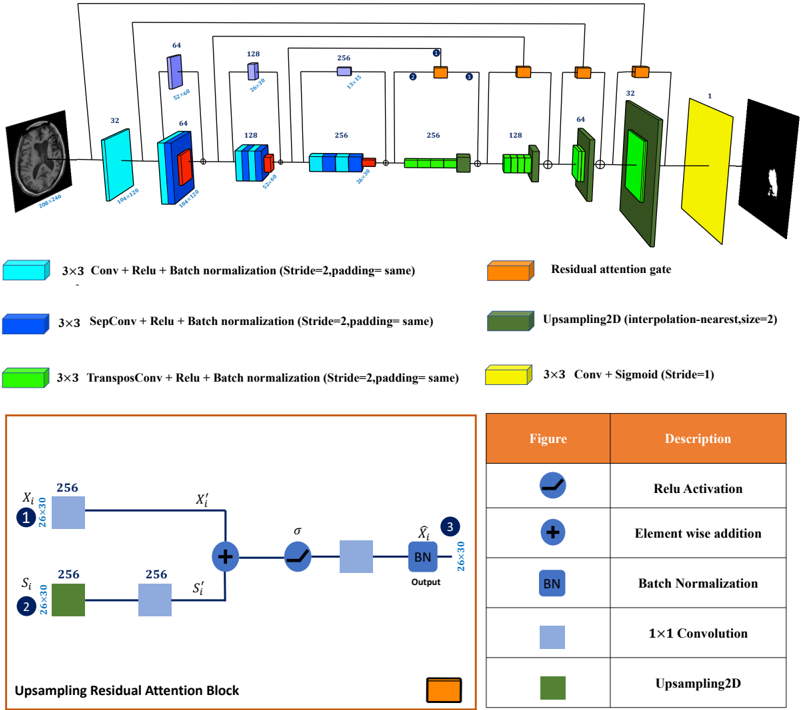
\includegraphics[width=0.9\linewidth]{../figures/figure_005.png}
\caption{Fig. 4. Architecture of the proposed RAX-Net, showing encoder-decoder design, residual connections, and residual attention blocks.}
\end{figure}
\begin{figure}[htbp]
\centering
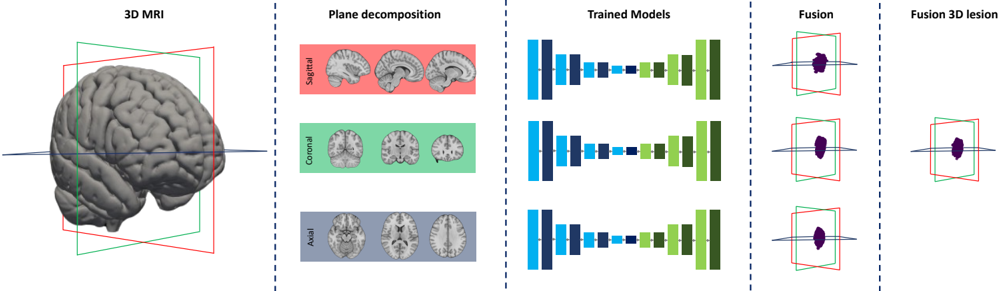
\includegraphics[width=0.9\linewidth]{../figures/figure_006.png}
\caption{Fig. 5. Workflow of the proposed approach: (i) decomposition of 3D MRI into 2D slices, (ii) per-plane lesion segmentation using 2D models, and (iii) aggregation of predictions into a final 3D mask.}
\end{figure}
\begin{figure}[htbp]
\centering
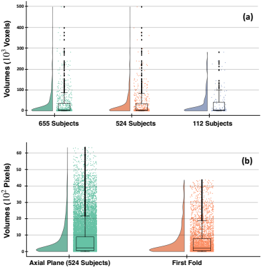
\includegraphics[width=0.9\linewidth]{../figures/figure_007.png}
\caption{Fig. 6. Lesion distributions in ATLAS v2.0. (a) Lesion voxel-size distribution for the 524 cases used to train/evaluate 2D models and the 112 cases reserved for aggregation and 3D segmentation. (b) Axialplane lesion pixel-size distribution for the 524-case set and for one representative cross-validation fold.}
\end{figure}
\begin{figure}[htbp]
\centering
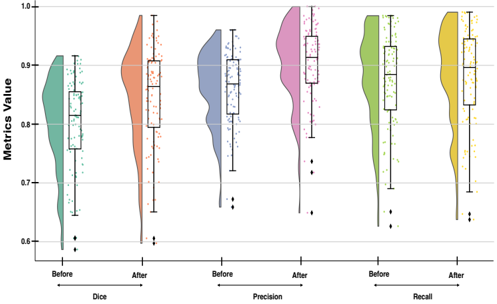
\includegraphics[width=0.9\linewidth]{../figures/figure_008.png}
\caption{Fig. 7. Axial-plane evaluation metrics before and after aggregation.}
\end{figure}
\begin{figure}[htbp]
\centering
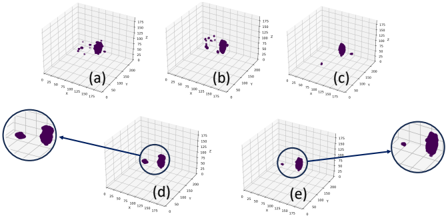
\includegraphics[width=0.9\linewidth]{../figures/figure_009.png}
\caption{Fig. 8. Representative 3D visualization: (a-c) planes (Axial, Sagittal, and Coronal), (d) ground-truth mask, and (e) final segmentation after aggregation.}
\end{figure}
\begin{figure}[htbp]
\centering
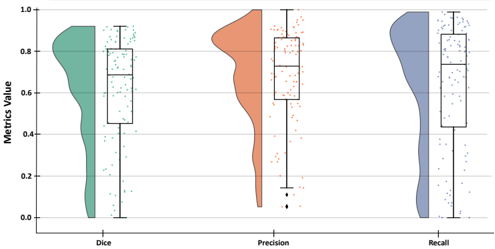
\includegraphics[width=0.9\linewidth]{../figures/figure_010.png}
\caption{Fig. 9. Raincloud plots of Dice, precision, and recall across 112 subjects.}
\end{figure}
\end{document}
